\documentclass[11pt]{article}

% Change "review" to "final" to generate the final (sometimes called camera-ready) version.
% Change to "preprint" to generate a non-anonymous version with page numbers.
\usepackage[review]{acl}

% Standard package includes
\usepackage{times}
\usepackage{latexsym}

% For proper rendering and hyphenation of words containing Latin characters (including in bib files)
\usepackage[T1]{fontenc}
% This assumes your files are encoded as UTF8
\usepackage[utf8]{inputenc}

% This is not strictly necessary, and may be commented out,
% but it will improve the layout of the manuscript,
% and will typically save some space.
\usepackage{microtype}

% This is also not strictly necessary, and may be commented out.
% However, it will improve the aesthetics of text in
% the typewriter font.
\usepackage{inconsolata}

% Including images in your LaTeX document requires adding
% additional package(s)
\usepackage{graphicx}
\usepackage{subcaption}
\usepackage{booktabs}

% Math
\usepackage{amsmath}
\usepackage{amssymb}
\usepackage{mathtools}
\usepackage{amsthm}
\usepackage{bbm}
\usepackage{enumitem}

% Algorithm packages
\usepackage{algorithm}
\usepackage{algorithmic}

% Colored symbols for tables
\usepackage{xcolor}
\usepackage{pifont}
\newcommand{\cmark}{\textcolor{green!80!black}{\ding{51}}}
\newcommand{\xmark}{\textcolor{red}{\ding{55}}}

% Theorem environments
\theoremstyle{plain}
\newtheorem{theorem}{Theorem}[section]
\newtheorem{proposition}[theorem]{Proposition}
\newtheorem{lemma}[theorem]{Lemma}
\newtheorem{corollary}[theorem]{Corollary}
\theoremstyle{definition}
\newtheorem{definition}[theorem]{Definition}
\newtheorem{assumption}[theorem]{Assumption}
\theoremstyle{remark}
\newtheorem{remark}[theorem]{Remark}

% Paper-specific commands
\newcommand{\papertitle}{Fast Block Diffusion Training via Multi-Mask Context Sharing}
\newcommand{\name}{MMT}
\newcommand{\NAME}{Multi-Mask Training}

\title{\papertitle}

\author{First Author \\
  Affiliation / Address line 1 \\
  Affiliation / Address line 2 \\
  Affiliation / Address line 3 \\
  \texttt{email@domain} \\\And
  Second Author \\
  Affiliation / Address line 1 \\
  Affiliation / Address line 2 \\
  Affiliation / Address line 3 \\
  \texttt{email@domain} \\}

\begin{document}
\maketitle

\begin{abstract}
  Block Diffusion Language Models generate multiple blocks of text sequentially, while tokens within each block are denoised in parallel, enabling efficient parallel decoding.
  However, their training suffers from low computational utilization: each sample is duplicated into a clean context and a masked copy, yet only the masked portion contributes to the training loss, resulting in merely 50\% effective computation.
  In this paper, we propose \textbf{\NAME{} with context sharing} (\textbf{\name{}}), a simple yet effective training paradigm that significantly improves computational efficiency through context sharing.
  Our key idea is to generate $K$ different mask patterns for the same clean text and process them together in a single forward pass via a sparse attention mechanism, where each masked segment attends to the shared clean context while remaining isolated from other segments.
  Notably, we observe that seeing each sample multiple times with different masks can match or surpass the quality of seeing more unique samples.
  We find $K{=}4$ to be optimal, which raises the effective utilization from 50\% to 80\% and yields a $1.6\times$ training speedup with no degradation in perplexity (TODO) or downstream performance.
\end{abstract}

\section{Introduction}

\begin{figure}[t]
    \centering
    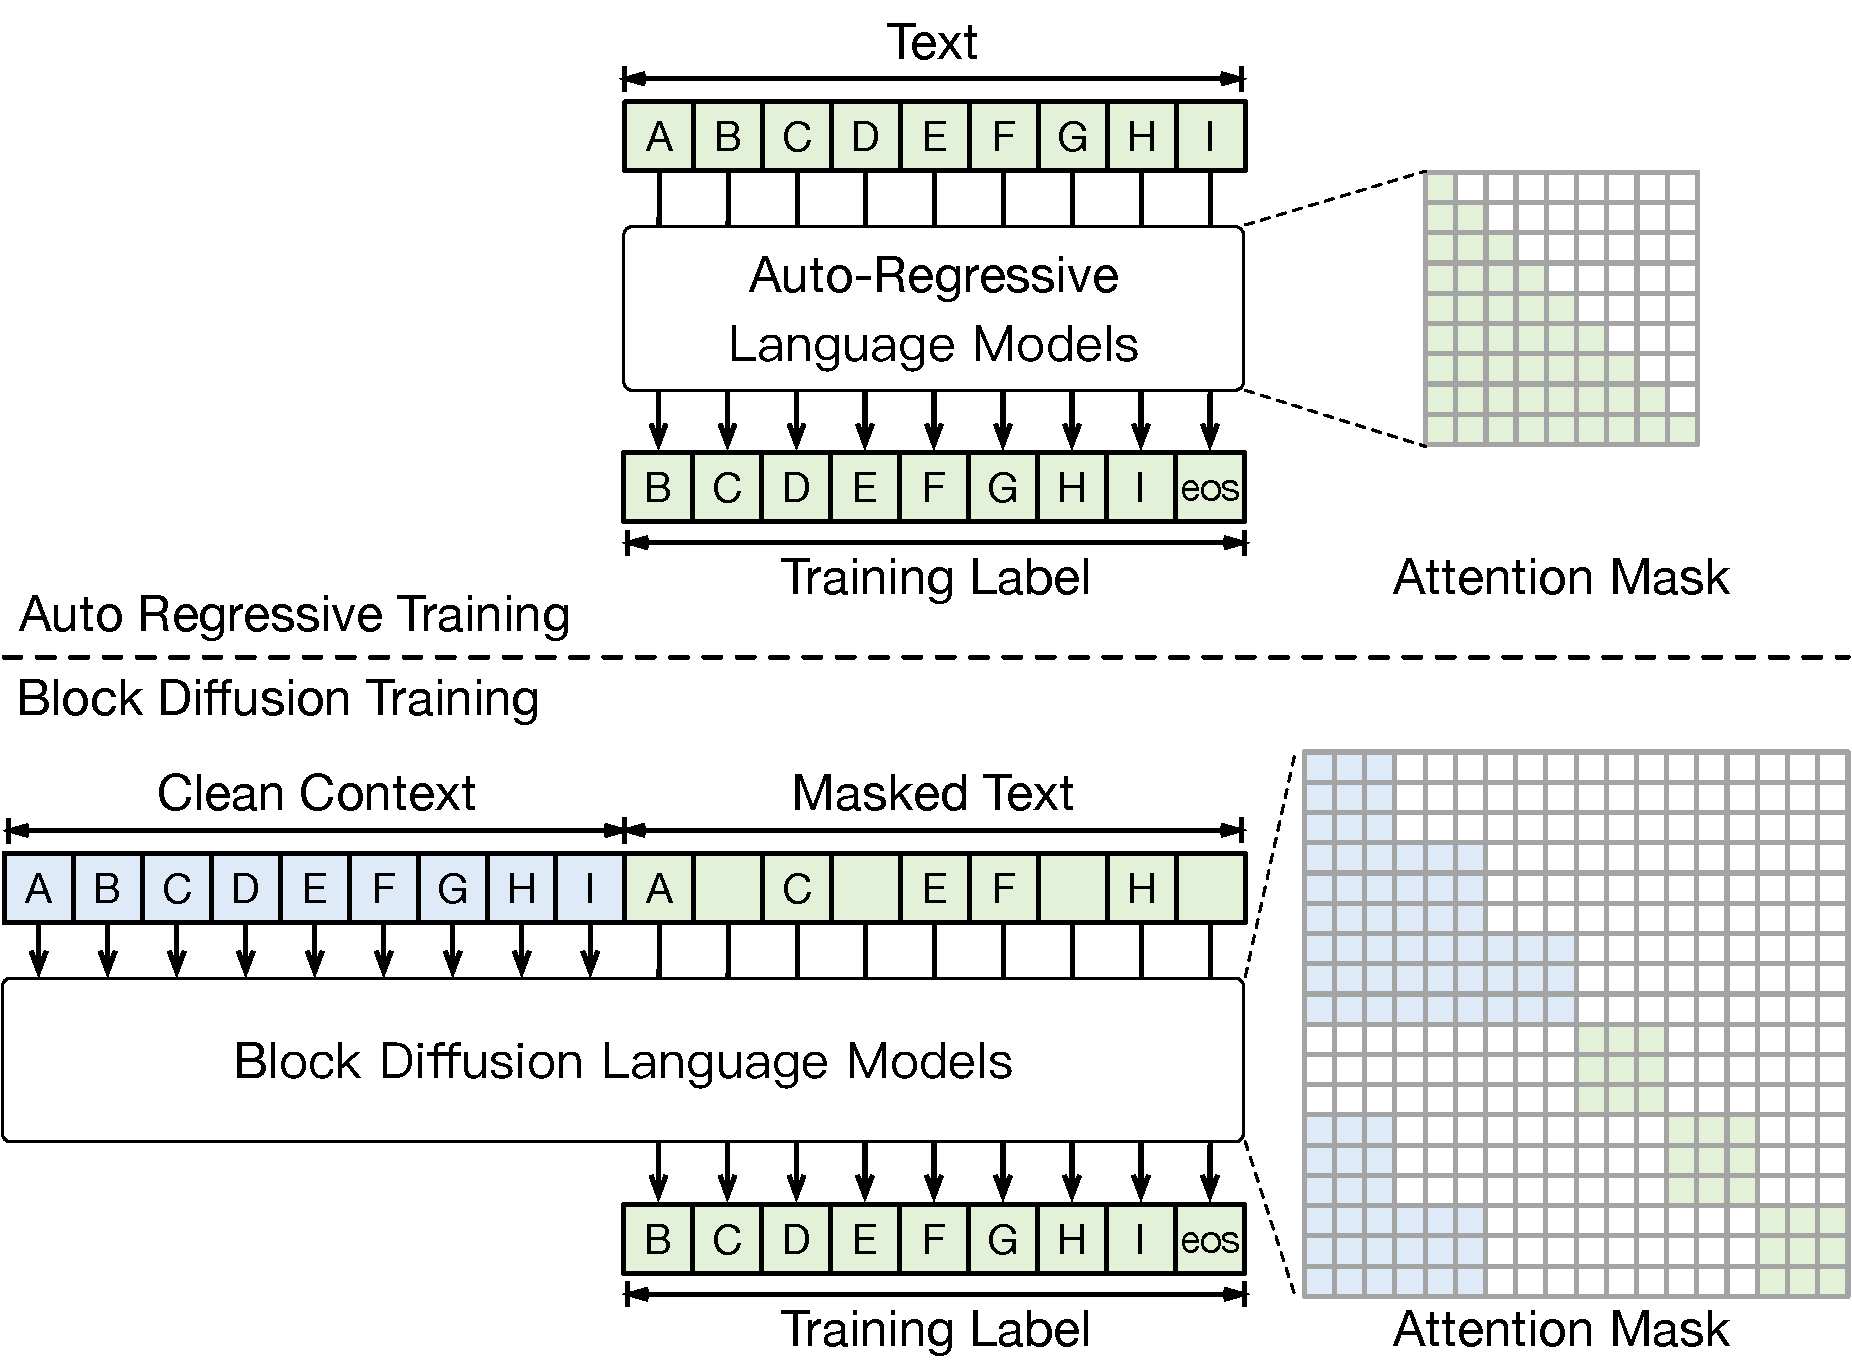
\includegraphics[width=0.47\textwidth]{figures/original_pattern.pdf}
    \caption{The training pattern of Auto-Regressive Language Models and Block Diffusion Language Models.}
    \label{fig:original_pattern}
\end{figure}

\begin{figure*}[t]
    \centering
    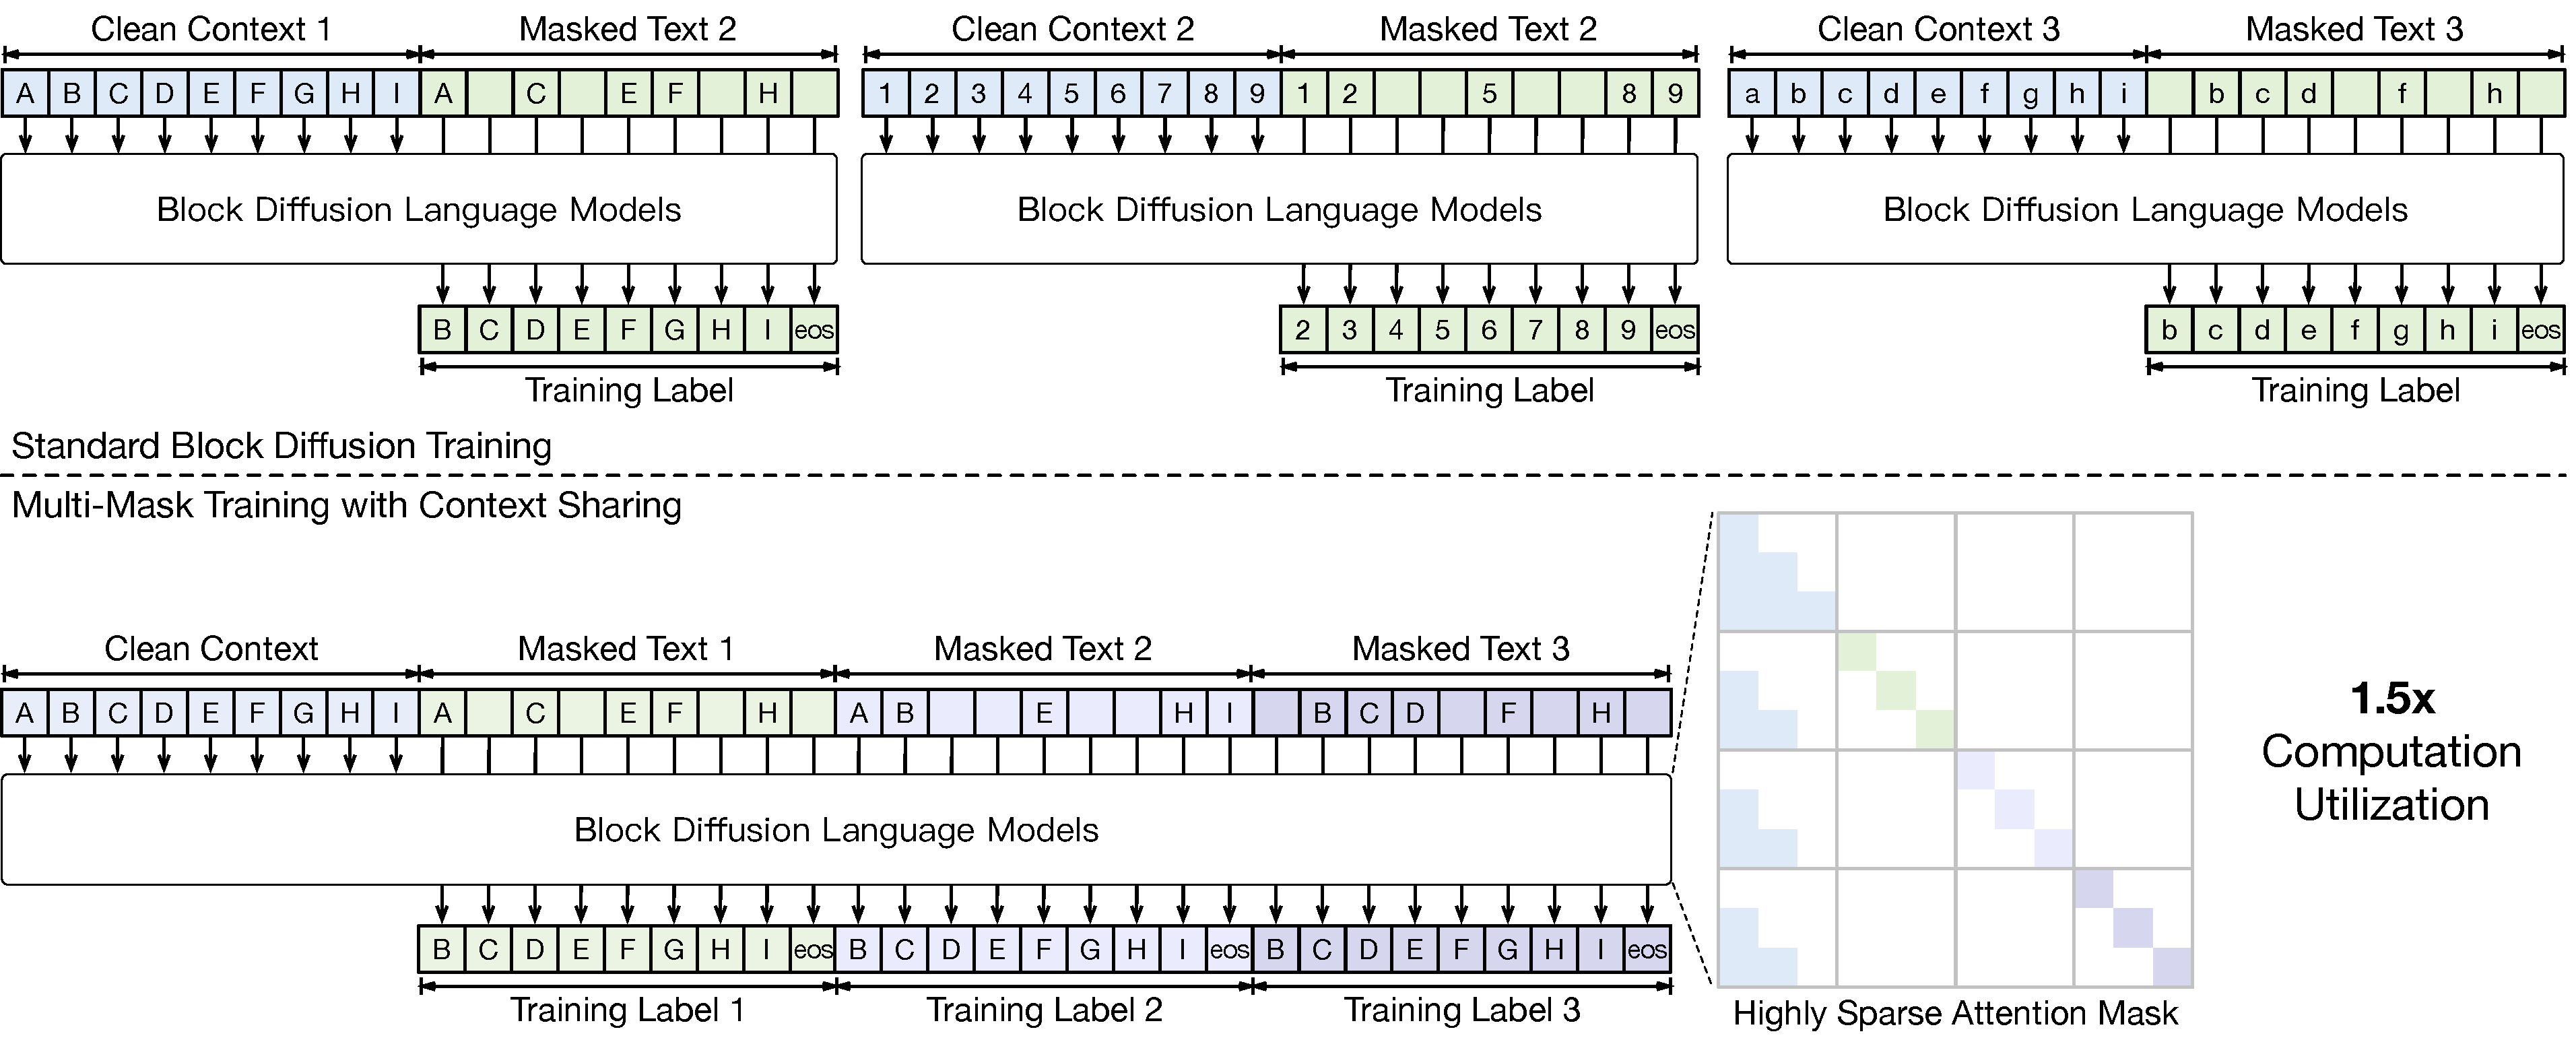
\includegraphics[width=0.95\textwidth]{figures/new_pattern.pdf}
    \caption{The training pattern of \name{} compared to the original training pattern of Block Diffusion Language Models, when the number of different mask patterns $K$ is $3$. MMT train on less training instance but instead train on more mask patterns.}
    \label{fig:method}
\end{figure*}

The success of Large Language Models~\citep{gpt3,foundation-model,PTMs-survey,gpt4} has been largely driven by autoregressive (AR) architectures.
However, their sequential, token-by-token generation paradigm imposes significant latency bottlenecks during inference.
Recently, Diffusion Language Models~\citep{llada,mercury,seeddiffusion,geminidiffusion} have emerged as promising alternatives.
By training the model to generate tokens in parallel, these models offer a flexible trade-off between generation quality and inference speed.

Block Diffusion Language Models~\citep{bd3lms,fastdllmv2,sdar,nbdiff,llada2} further bridge the gap between autoregressive and diffusion paradigms.
These models decompose the generation process into sequential blocks, where tokens within each block are generated via diffusion while blocks themselves are produced autoregressively.
This hybrid formulation enables variable-length generation, supports KV caching across blocks, and allows parallel token sampling within each block, making it a compelling architecture for practical deployment.

Despite their promising inference properties, Block Diffusion Language Models suffer from a critical training inefficiency.
As illustrated in Figure~\ref{fig:original_pattern}, each training sample is duplicated into two copies: one serves as the clean context, while the other is masked and used for loss computation.
This duplication results in a mere 50\% computational utilization, as half of the forward pass is spent on the context that does not contribute to the training signal.
In contrast, autoregressive models achieve near-100\% utilization since every token contributes to the training loss.
Beyond the wasted FLOPs, this inefficiency also incurs substantial memory and I/O overhead: the clean context occupies precious GPU memory during forward and backward passes, yet contributes zero gradients to the model update.

In this paper, we propose \textbf{\NAME{} with context sharing} (\textbf{\name{}}), a simple yet effective training paradigm that significantly improves computational utilization through a carefully designed attention mechanism.
Our key insight is that instead of processing one mask pattern per sample, we can generate $K$ different mask patterns for the same clean text and process them together in a single forward pass.
As illustrated in Figure~\ref{fig:method}, by concatenating the shared clean prefix with $K$ masked suffixes and employing a \emph{context-sharing attention mask}, each masked segment attends to the clean context while remaining isolated from other segments.
The resulting attention mask is highly sparse and can be efficiently implemented with FlexAttention~\citep{flexattention}.
This design amortizes the cost of the clean context across $K$ perturbations, improving the computational utilization from $50\%$ to $\frac{K}{1+K}$.
Crucially, we find that when using appropriate number of mask patterns $K$, \textbf{training on fewer samples with multiple perturbations per sample} yields comparable or even better model quality than training on more samples with single perturbations.
Intuitively, by exposing the model to $K$ different mask patterns of the same underlying text within a single forward pass, \name{} acts as an implicit ensemble over perturbations, reducing the variance of the gradient signal and leading to more stable optimization.
This \emph{variance reduction} effect explains why \name{} can achieve faster training without sacrificing or even improving model quality.

Beyond training, our context-sharing attention mask can also accelerate inference in diffusion-based reinforcement learning (RL).
In diffusion RL, evaluating the probability of generated text requires Monte-Carlo sampling over multiple mask patterns, which is computationally expensive when performed naively.
By batching these mask patterns together and applying our sparse attention mechanism, we can significantly reduce the cost of probability estimation during policy optimization.

Our contributions are summarized as follows:
\begin{itemize}[parsep=0pt,itemsep=3pt,topsep=0pt]
    \item We identify the low computational utilization in Block Diffusion training, where the clean context incurs computation but does not contribute to the loss.
    \item We propose \name{}, a multi-mask training paradigm with context sharing that processes multiple masked perturbations of the same sample in a single forward pass via a specially designed sparse attention pattern.
    \item Experiments show that \name{} accelerates Block Diffusion training by $1.6\times$ with no loss in perplexity (TODO) or downstream task performance.
\end{itemize}

\section{Related Work}

\subsection{Diffusion Language Models}
Diffusion models have achieved remarkable success in continuous domains such as image and audio generation~\citep{sohl2015deep,ddpm,song2020score,dit}.
Recently, there has been growing interest in adapting diffusion-based methods to discrete text generation. Mercury~\citep{mercury}, Seed Diffusion~\citep{seeddiffusion}, and Gemini Diffusion~\citep{geminidiffusion} are industry-developed diffusion language models that demonstrate ultra-fast inference capabilities.
In the open-source community, early methods~\citep{li2022diffusion,lovelace2023latent,gong2022diffuseq,han2023ssd,strudel2022self,chen2022analog} applies continious space diffusion directly to language,
while more recent methods~\citep{hoogeboom2021argmax,hoogeboomautoregressive,he2023diffusionbert,loudiscrete,ou2024your,sahoo2024simple} leverage discrete diffusion to achieve better scalability and performance.
In this paper, we mainly focus on the discrete version, also known as \textbf{masked diffusion language models}.
LLaDA~\citep{llada} trains an 8B-scale masked diffusion language model from scratch, demonstrating competitive performance with autoregressive counterparts.
DREAM~\citep{dream} adapts pre-trained autoregressive models into diffusion language models through continued training.
These methods offer a promising alternative to autoregressive generation by enabling parallel token sampling, but they typically generate sequences of fixed length and lack the flexibility of variable-length generation.

\subsection{Block Diffusion Language Models}
Block Diffusion Language Models bridge the gap between autoregressive and diffusion paradigms by decomposing generation into sequential blocks.
\citet{ma2025dkv,wu2025fast} use approximate KV caching to make a diffusion language model generate block-by-block.
BD3-LMs~\citep{bd3lms} trains a native block diffusion language model from scratch.
Fast-DLLM v2~\citep{fastdllmv2} and SDAR~\citep{sdar} adapt pre-trained autoregressive models into block diffusion models, enabling efficient conversion of existing AR checkpoints.
LLaDA 2.0~\citep{llada2} scales block diffusion language models up to 100B parameters, demonstrating the scalability of this approach.
These models support variable-length generation, enable KV caching across blocks, and allow parallel token sampling within each block.
However, their training suffers from low computational utilization due to the context duplication, which our method addresses.

\subsection{Data Efficiency of Diffusion Language Models}
Recent studies~\citep{prabhudesaidiffusion,ni2025diffusion,ni2025training} have revealed that diffusion language models are ``super data learners'' that can extract more information from the same amount of training data through diverse mask patterns.
Another related approach is \emph{complementary masking}~\citep{fastdllmv2}, which uses an inverted mask paired with a standard mask to enhance data utilization.
However, these methods suffer from efficiency drawbacks.
The former relies on implicit accumulation of diversity over repeated epochs with single-mask sampling,
while the latter doubles the batch size and processes each perturbation independently, failing to exploit the shared clean context.
In contrast, our method transforms this implicit benefit into an explicit, efficient training strategy.
By processing multiple mask patterns simultaneously with \textbf{context sharing}, we actively enforce diverse supervision within each step while eliminating the computational waste of encoding the same context repeatedly.

\section{Method}

\subsection{Preliminaries}

\paragraph{Notation.}
Let $\mathbf{x} = (x_1, x_2, \ldots, x_N)$ denote a sequence of $N$ tokens, and let $\mathtt{M}$ denote the special mask token.
We denote the parameter of language model as $\theta$.
Notably, both autoregressive and diffusion-based language models share the same Transformer architecture, they differ only in their input representations and training objectives.

\paragraph{Autoregressive Language Models.}
Autoregressive (AR) language models is trained to minimize the negative log-likelihood of the sequence:
\begin{equation}
    \mathcal{L}_{\text{AR}} = -\mathbb{E}_{\mathbf{x} \sim \mathcal{D}} \left[ \sum_{i=1}^{N} \log p_{\theta}(x_i \mid x_{<i}) \right].
\end{equation}

\paragraph{Masked Diffusion Language Models.}
Masked diffusion language models (MDLMs)~\citep{llada} define a discrete diffusion process over token sequences.
Let $t\sim\mathcal{U}(0,1)$ denote a noise level, and let
$\mathbf{x}^t$ denote the corrupted sequence obtained by independently
masking each token $x_i$ with probability $t$.
Formally, for each position $i$:
\begin{equation}
    x_i^{t} =
    \begin{cases}
        \mathtt{M} & \text{with probability } t, \\
        x_i & \text{otherwise}.
    \end{cases}
\end{equation}
The model is trained to predict the original tokens from the corrupted sequence:
\begin{equation}
\begin{aligned}
&\mathcal{L}_{\mathrm{MDLM}}
=
-\mathbb{E}_{t,\mathbf{x},\mathbf{x}^{t}}
\left[
\frac{1}{t}
\sum_{i=1}^{N}
\mathbb{I}\!\left[x_i^{t}=\mathtt{M}\right]
\ell_{\theta,i}^{\mathrm{MDLM}}(t)
\right], \\
&\ell_{\theta,i}^{\mathrm{MDLM}}(t)
=
\log p_{\theta}
\left(
x_i
\,\middle|\,
\mathbf{x}^{t}
\right).
\end{aligned}
\label{eq:mdlm_loss}
\end{equation}


\paragraph{Block Diffusion Language Models.}
Block diffusion language models (BDLMs)~\citep{bd3lms} extend MDLMs by
partitioning the sequence into contiguous blocks of size $B$.
The sequence is divided into $N_b=N/B$ blocks,
$\mathbf{x}=(\mathbf{b}_1,\ldots,\mathbf{b}_{N_b})$.
During training, each block $r\in\{1,\ldots,N_b\}$ is assigned an
independently sampled noise level $t_r\sim\mathcal{U}(0,1)$.
Tokens within $\mathbf{b}_r$ are then masked independently with probability
$t_r$, while the causal structure across blocks is maintained.
For each token $x_i$, let
$j=\lceil i/B\rceil$
denote its block index in the following objective:

\begin{equation}
\begin{aligned}
&\mathcal{L}_{\mathrm{BDLM}}
=
-\mathbb{E}_{\boldsymbol{t},\mathbf{x},\mathbf{x}^{\boldsymbol{t}}}
\left[
\sum_{i=1}^{N}
\frac{
\mathbb{I}\!\left[x_i^{\boldsymbol{t}}=\mathtt{M}\right]
}{
t_j
}
\ell_{\theta,i}^{\mathrm{BDLM}}(t_j)
\right], \\
&
\ell_{\theta,i}^{\mathrm{BDLM}}(t_j)
=
\log p_{\theta}
\left(
x_i
\,\middle|\,
\mathbf{b}_{<j},
\mathbf{b}_{j}^{t_j}
\right).
\end{aligned}
\label{eq:bdlm_loss}
\end{equation}

where $\mathbf{b}_{<j}$ denotes the clean preceding blocks in $\mathbf{x}$, and $\mathbf{b}_{j}^{t}$ denotes the noisy version of the $j$-th block in $\mathbf{x}^{t}$. The specialized attention mask used for efficient BDLM training is illustrated in Figure~\ref{fig:original_pattern}.

\subsection{\name{}: \NAME{}}

\paragraph{Training formulation}
Given a sequence $\mathbf{x}$, we sample $K$ independent noise levels $t_1, t_2, \ldots, t_K \in [0, 1]$ and generate $K$ corresponding corrupted sequences $\mathbf{x}^{t_1}, \mathbf{x}^{t_2}, \ldots, \mathbf{x}^{t_K}$.
The training objective of \name{} is:
\begin{equation}
\begin{aligned}
    &\mathcal{L}_{\text{\name{}}} = -\mathbb{E}_{\{t_k\}_{k=1}^K, \mathbf{x}, \{\mathbf{x}^{t_k}\}_{k=1}^K} \Bigg[\\
    &{1\over K}\sum_{k=1}^K {1\over t_k} \sum_{i=1}^N [x_i^{t_k} = \mathtt{M}] \log p_{\theta}(x_i \mid \mathbf{b}_{<block(i)}, \mathbf{b}_{block(i)}^{t_k}) \Bigg].
\end{aligned}
\end{equation}

\paragraph{Training formulation}
Given a clean sequence $\mathbf{x}$, \name{} shares this clean sequence as the common context and generates $K$ corrupted sequences for denoising training.
For each view $k\in\{1,\ldots,K\}$, a noise level $t_k\sim\mathcal{U}(0,1)$ is independently sampled, and the corresponding corrupted sequence $\mathbf{x}^{t_k}$ is generated by masking each token with probability $t_k$.
The training objective averages the denoising losses over these $K$ noised views:
\begin{equation}
\begin{aligned}
&\mathcal{L}_{\mathrm{MMT}}
=
\mathbb{E}
\left[
\frac{1}{K}
\sum_{k=1}^{K}
\mathcal{J}_{k}(\mathbf{x})
\right], \\
&\mathcal{J}_{k}(\mathbf{x})
=
-\frac{1}{t_k}
\sum_{i=1}^{N}
\mathbb{I}\!\left[x_i^{t_k}=\mathtt{M}\right]
\ell_{\theta,i}^{\mathrm{MMT}}(t_k), \\
&\ell_{\theta,i}^{\mathrm{MMT}}(t_k)
=
\log p_{\theta}
\left(
x_i
\,\middle|\,
\mathbf{b}_{<j},
\mathbf{b}_{j}^{t_k}
\right).
\end{aligned}
\label{eq:mmt_loss}
\end{equation}
where the expectation is taken over $\mathbf{x}$, the independently sampled noise levels $\{t_k\}_{k=1}^{K}$, and the corresponding corrupted sequences $\{\mathbf{x}^{t_k}\}_{k=1}^{K}$.
Here, $j$ denotes the block index of token $x_i$, $\mathbf{b}_{<j}$ denotes the clean preceding blocks shared by all noised views, and $\mathbf{b}_{j}^{t_k}$ denotes the noisy version of the $j$-th block in the $k$-th corrupted sequence.

where the expectation is taken over $\mathbf{x}$, the block-wise noise levels
$\{\boldsymbol{t}_k\}_{k=1}^{K}$, and the corresponding corrupted views
$\{\mathbf{x}^{\boldsymbol{t}_k}\}_{k=1}^{K}$.
The block notation follows Eq.~\eqref{eq:bdlm_loss}, while
$t_{k,j}$ denotes the noise level assigned to block $j$ in the $k$-th corrupted view.

\paragraph{Context-sharing attention mechanism}
To enable efficient parallel training of all $K$ perturbations while maintaining correct token visibility, we construct an attention mask $\mathbf{M} \in \{0, 1\}^{(K+1)N \times (K+1)N}$ over token indices.
We use $k = 0$ for the clean sequence $\mathbf{x}$ and $k \in \{1, \ldots, K\}$ to index the $K$ perturbations $\mathbf{x}^{t_k}$.
Let $(k, i)$ denote the $i$-th token of the $k$-th sequence.
The attention mask entry $M_{(k,i), (k',i')}$ determines whether token $(k,i)$ can attend to token $(k',i')$:
\begin{equation}
    M_{(k,i), (k',i')} =
    \begin{cases}
        1, & \text{if } k' = 0 \text{ and } \lceil i' / B \rceil < \lceil i / B \rceil, \\
        1, & \text{if } k' = k \text{ and } \lceil i' / B \rceil = \lceil i / B \rceil, \\
        0, & \text{otherwise}.
    \end{cases}
\label{eq:attn_mask}
\end{equation}
This mask ensures that each perturbation can attend to: (1) preceding blocks from the shared clean sequence, and (2) its own noisy block at the current position.
The efficient training mask of \name{} is illustrated in Figure~\ref{fig:method}.

\paragraph{Complementary masking via Context Sharing.}
We adopt the complementary masking strategy~\citep{fastdllmv2}.
Instead of independently sampling $K$ mask patterns, we sample $K/2$ pairs of complementary mask patterns.
Crucially, unlike prior implementations that double the context computation cost, our context-sharing paradigm allows us to process complementary masks against a single clean context representation.
 The training objective of \name{} becomes:
\begin{equation}
    \mathcal{L}_{\text{\name{}}} = -\mathbb{E}_{\{t_j\}_{j=1}^{K/2}, \mathbf{x}, \{\mathbf{x}^{t_j}\}_{j=1}^{K/2}} \Bigg[
    \frac{1}{K} \sum_{j=1}^{K/2} \mathcal{L}_{\text{pair}}^{(j)}\Bigg].
\end{equation}
Each pair of complementary masks consist an inverse mask patterns $m$ and $\bar m= 1-m$, generating two noisy sequece $\mathbf{x}^{t_j}$ and $\bar{\mathbf{x}}^{t_j}$, where
\begin{equation}
    \bar{x}_i^{t_j} =
    \begin{cases}
        x_i & \text{if } x_i^{t_j} = \mathtt{M}, \\
        \mathtt{M} & \text{otherwise}.
    \end{cases}
\end{equation}
The paired loss is then defined as
\begin{equation}
\begin{aligned}
    \mathcal{L}_{\text{pair}}^{(j)} = & \sum_{i=1}^N [x_i^{t_j} = \mathtt{M}] \log p_{\theta}(x_i \mid \mathbf{b}_{<block(i)}, \mathbf{b}_{block(i)}^{t_j}) \\
    + & \sum_{i=1}^N [\bar{x}_i^{t_j} = \mathtt{M}] \log p_{\theta}(x_i \mid \mathbf{b}_{<block(i)}, \bar{\mathbf{b}}_{block(i)}^{t_j}) \Bigg],
\end{aligned}
\end{equation}
where $\bar{\mathbf{b}}^{t_j}_{block(i)}$ is the $i$-th noisy blocks of $\bar{\mathbf{x}}^{t_j}$. We eliminate the normalization factor $1/t_j$ following \citet{fastdllmv2}, as the complementary masks jointly cover all $N$ tokens.

\paragraph{Training algorithm.}
We summarize the complete training procedure of \name{} in Algorithm~\ref{alg:mmt}.

(Working in Progress...)

\begin{algorithm}[t]
\caption{\name{} Training}
\label{alg:mmt}
\begin{algorithmic}[1]
\REQUIRE Model $p_\theta$, dataset $\mathcal{D}$, number of mask pairs $K/2$, block size $B$
\FOR{each training iteration}
    \STATE Sample minibatch $\{\mathbf{x}\}$ from $\mathcal{D}$
    \STATE \textcolor{gray}{\textit{// Generate K complementary mask pairs}}
    \FOR{$j = 1$ to $K/2$}
        \STATE Sample $t_j \sim \text{Uniform}(0, 1)$
        \STATE Sample $\mathbf{m}_j \in \{0,1\}^N$, $m_{j,i} \sim \text{Bernoulli}(t_j)$
        \STATE $\mathbf{x}^{t_j} \gets \mathbf{x} \odot (1 - \mathbf{m}_j) + \mathtt{M} \odot \mathbf{m}_j$
        \STATE $\bar{\mathbf{x}}^{t_j} \gets \mathbf{x} \odot \mathbf{m}_j + \mathtt{M} \odot (1 - \mathbf{m}_j)$
    \ENDFOR
    \STATE \textcolor{gray}{\textit{// Construct input with shared clean context}}
    \STATE $\mathbf{X} \gets \text{Concat}(\mathbf{x}, \mathbf{x}^{t_1}, \bar{\mathbf{x}}^{t_1}, \ldots, \mathbf{x}^{t_{K/2}}, \bar{\mathbf{x}}^{t_{K/2}})$
    \STATE Construct attention mask $\mathbf{M}$ per Eq.~(\ref{eq:attn_mask})
    \STATE \textcolor{gray}{\textit{// Forward and backward pass}}
    \STATE $\mathcal{L} \gets \mathcal{L}_{\text{\name{}}}(p_\theta(\mathbf{X}; \text{attn\_mask}=\mathbf{M}))$
    \STATE Update $\theta$ via gradient descent on $\mathcal{L}_{\text{\name{}}}$
\ENDFOR
\end{algorithmic}
\end{algorithm}

\subsection{Computational Complexity Analysis}

We analyze the computational complexity of different language modeling paradigms.
Let $N$ denote the sequence length, $P$ the total model parameters, $L$ the number of transformer layers, and $d$ the hidden dimension.

\paragraph{Per-token training cost.}
Following \citet{chen-etal-2025-cost}, the FLOPs required to process one token with context length $n$ is:
\begin{equation}
    C_{\text{token}}(n) = \underbrace{2P}_{\text{non-attention}} + \underbrace{4n L d}_{\text{attention}}.
\end{equation}
Here $n$ is the number of visible tokens in the masked attention mechanism.

\paragraph{Autoregressive Transformers.}
For causal language models generating a sequence of length $N$, the total FLOPs is:
\begin{equation}
\begin{aligned}
    C_{\text{AR}} &= \sum_{t=1}^{N} C_{\text{token}}(t) = 2PN + \sum_{t=1}^{N} 4t L d \\
    &= \underbrace{2PN}_{\text{non-attention}} + \underbrace{2N(N+1) L d}_{\text{attention}}.
\end{aligned}
\end{equation}

\paragraph{Block Diffusion Language Models.}
Block diffusion models partition the sequence into $N_b = N / B$ blocks.
At block $j$ of the clean sequence $\mathbf{x}$, the model attends to all $(j-1)B$ preceding tokens plus the current block of size $B$.
At block $j$ of the noisy sequence $\mathbf{x}^{t}$, the model attends to all $(j-1)B$ preceding clean tokens plus the current noisy block of size $B$.
That is, the $j$-th block of each sequence attends to $jB$ tokens.
The total FLOPs is
\begin{equation}
\begin{aligned}
    C_{\text{BDLM}} &= 2 \sum_{i=1}^{N} C_{\text{token}}((\lceil i/B \rceil)B) \\
    &= 2 \sum_{j=1}^{N_b} B \cdot C_{\text{token}}(jB) \\
    &= 2 (2P N_b B + 2 B^2 N_b(N_b+1) L d) \\
    &= 2\times \left(\underbrace{2PN}_{\text{non-attention}} + \underbrace{2N(N+B) L d}_{\text{attention}}\right).
\end{aligned}
\end{equation}

\paragraph{\name{} (Ours).}
Our context-sharing mechanism processes the clean context once and shares it across $K$ perturbations.
Similar to the above, we process $1+K$ sequences in total, where the $j$-th block of each sequence attends to $jB$ tokens.
The total FLOPs is
\begin{equation}
\begin{aligned}
    C_{\text{\name{}}} &= (1+K) \sum_{j=1}^{N_b} B \cdot C_{\text{token}}(jB) \\
    &= (1+K) \times \left(\underbrace{2PN}_{\text{non-attention}} + \underbrace{2N(N+B) L d}_{\text{attention}}\right).
\end{aligned}
\end{equation}
The amortized cost per perturbation is:
\begin{equation}
    \frac{C_{\text{\name{}}}}{K} = (1+1/K) \times \left(\underbrace{2PN}_{\text{non-attention}} + \underbrace{2N(N+B) L d}_{\text{attention}}\right).
\end{equation}

In typical training settings, the sequence length $N$ is at least 2048 or 4096, while the block size $B$ is usually set to small values such as 32 or 64~\citep{fastdllmv2}.
Since $B \ll N$, we have $N(N+B) \approx N^2$ and $N(N+1) \approx N^2$.
Table~\ref{tab:flops_comparison} summarizes the average training FLOPs per noise perturbation under this approximation.
As shown, \name{} significantly improves the FLOPs efficiency compared to block diffusion, which can be viewed as a special case of our method with $K=1$.

\begin{table}[h]
\centering
\caption{Average FLOPs per sequence/perturbation. For \name{}, the cost is amortized over $K$ perturbations, and $(1+1/K) \approx 1$ when $K$ is reasonably large.}
\label{tab:flops_comparison}
\scalebox{0.9}{
\begin{tabular}{l|ccc}
\toprule
 & AR & BDLM & \name{} (Ours) \\
\midrule
Non-attention & $2PN$ & $4PN$ & $(1+1/K) \cdot 2PN$ \\
Attention & $2N^2 Ld$ & $4N^2 Ld$ & $(1+1/K) \cdot 2N^2 Ld$ \\
\bottomrule
\end{tabular}
}
\end{table}

-\section{Experiment}

We conduct experiments under two distinct training paradigms, ``AR to Diffusion'' and ``Training Diffusion from Scratch'', to comprehensively evaluate our proposed method.

\subsection{AR to Diffusion}

For \textbf{AR to Diffusion} experiments, we adopt the experimental settings and framework from Fast-dLLM v2~\citep{fastdllmv2} and use it as our baseline to evaluate the performance gains achieved by our proposed improvements.

\paragraph{Models}

We initialize our model from Qwen2.5-1.5B-Instruct~\citep{qwen2.5} and fine-tune it into a block diffusion language model following the training recipe of Fast-dLLM v2~\citep{fastdllmv2}.
The fine-tuning is performed on approximately 3B tokens sampled from the LLaMA-Nemotron post-training dataset~\citep{nemotronpost}.
The block size $B$ is set to 32, the batch size is set to $256$ and the context length is set to $2048$.
The learning rate is set to $2e-5$.

\paragraph{Benchmarks}

We conduct evaluation on MMLU~\citep{mmlu} and GPQA~\citep{gpqa} benchmarks for general ability evaluation.
We conduct evaluation on GSM8K~\citep{gsm8k}, MATH~\citep{math}, MBPP~\citep{mbpp}, and HumanEval~\citep{humaneval} benchmarks for mathematical reasoning and code generation tasks.
All benchmarks are evaluated in the zero-shot setting except that MMLU is evaluated in the 5-shot setting.

\paragraph{Results}

% TODO 表格里评测集加粗一下
\begin{table*}[t]
\centering
\caption{Comparison of different $K$ settings of \name{} in AR to Diffusion setting.}
\label{tab:ar2diff_main_results}
\scalebox{0.90}{
\begin{tabular}{l|ccccccc|c}
\toprule
Method & GSM8K & MATH & MMLU & GPQA & IFEval & MBPP & HumanEval & Avg. \\ % & Speedup
\midrule
$K$=1, 12000 steps & 64.54$_{\pm 1.48}$ & 29.74$_{\pm 0.14}$ & 49.51$_{\pm 1.48}$ & 26.27$_{\pm 0.91}$ & 41.47$_{\pm 1.07}$ & 46.95$_{\pm 2.87}$ & 45.32$_{\pm 1.54}$ & 43.40$_{\pm 0.43}$ \\ % & 1.00$\times$
\midrule
$K$=2, 6000 steps & 63.43$_{\pm 1.75}$ & 30.96$_{\pm 0.19}$ & 50.73$_{\pm 0.77}$ & 26.49$_{\pm 0.46}$ & 41.03$_{\pm 1.39}$ & 50.06$_{\pm 1.25}$ & 40.45$_{\pm 3.46}$ & 43.31$_{\pm 0.25}$ \\ % & 1.33$\times$
$K$=1, 6000 steps & 61.99$_{\pm 0.58}$ & 28.29$_{\pm 0.68}$ & 51.17$_{\pm 0.51}$ & 26.56$_{\pm 0.00}$ & 42.70$_{\pm 1.82}$ & 46.95$_{\pm 0.23}$ & 38.41$_{\pm 2.20}$ & 42.30$_{\pm 0.25}$ \\ % & 2.00$\times$
\midrule
$K$=4, 3000 steps & 62.25$_{\pm 0.89}$ & 29.32$_{\pm 0.47}$ & 51.60$_{\pm 0.25}$ & 26.86$_{\pm 0.52}$ & 42.70$_{\pm 1.30}$ & 48.12$_{\pm 0.60}$ & 42.68$_{\pm 1.61}$ & 43.36$_{\pm 0.13}$ \\ % & 1.60$\times$
$K$=1, 3000 steps & 59.21$_{\pm 0.72}$ & 25.85$_{\pm 0.74}$ & 52.39$_{\pm 0.22}$ & 26.41$_{\pm 0.68}$ & 41.90$_{\pm 0.93}$ & 46.95$_{\pm 2.38}$ & 35.17$_{\pm 1.96}$ & 41.13$_{\pm 0.07}$ \\ % & 4.00$\times$
\midrule
$K$=6, 2000 steps & 62.37$_{\pm 0.37}$ & 28.01$_{\pm 0.64}$ & 52.24$_{\pm 0.29}$ & 27.09$_{\pm 0.65}$ & 40.73$_{\pm 1.76}$ & 48.12$_{\pm 0.81}$ & 40.85$_{\pm 2.11}$ & 42.78$_{\pm 0.29}$ \\ % & 1.71$\times$
$K$=1, 2000 steps & 58.45$_{\pm 0.08}$ & 24.76$_{\pm 0.58}$ & 52.43$_{\pm 0.22}$ & 26.56$_{\pm 0.23}$ & 41.16$_{\pm 2.62}$ & 43.45$_{\pm 3.14}$ & 33.95$_{\pm 1.27}$ & 40.11$_{\pm 0.75}$ \\ % & 6.00$\times$
\midrule
$K$=8, 1500 steps & 61.46$_{\pm 1.03}$ & 27.83$_{\pm 0.69}$ & 52.56$_{\pm 0.38}$ & 26.86$_{\pm 0.68}$ & 41.71$_{\pm 3.62}$ & 47.60$_{\pm 0.81}$ & 38.62$_{\pm 2.14}$ & 42.38$_{\pm 0.45}$ \\ % & 1.78$\times$
$K$=1, 1500 steps & 56.03$_{\pm 0.35}$ & 23.97$_{\pm 0.41}$ & 52.74$_{\pm 0.13}$ & 27.38$_{\pm 0.13}$ & 39.99$_{\pm 2.78}$ & 43.58$_{\pm 1.17}$ & 34.96$_{\pm 2.14}$ & 39.81$_{\pm 0.74}$ \\ % & 8.00$\times$
\bottomrule
\end{tabular}
}
\end{table*}

\begin{figure}[t]
\centering
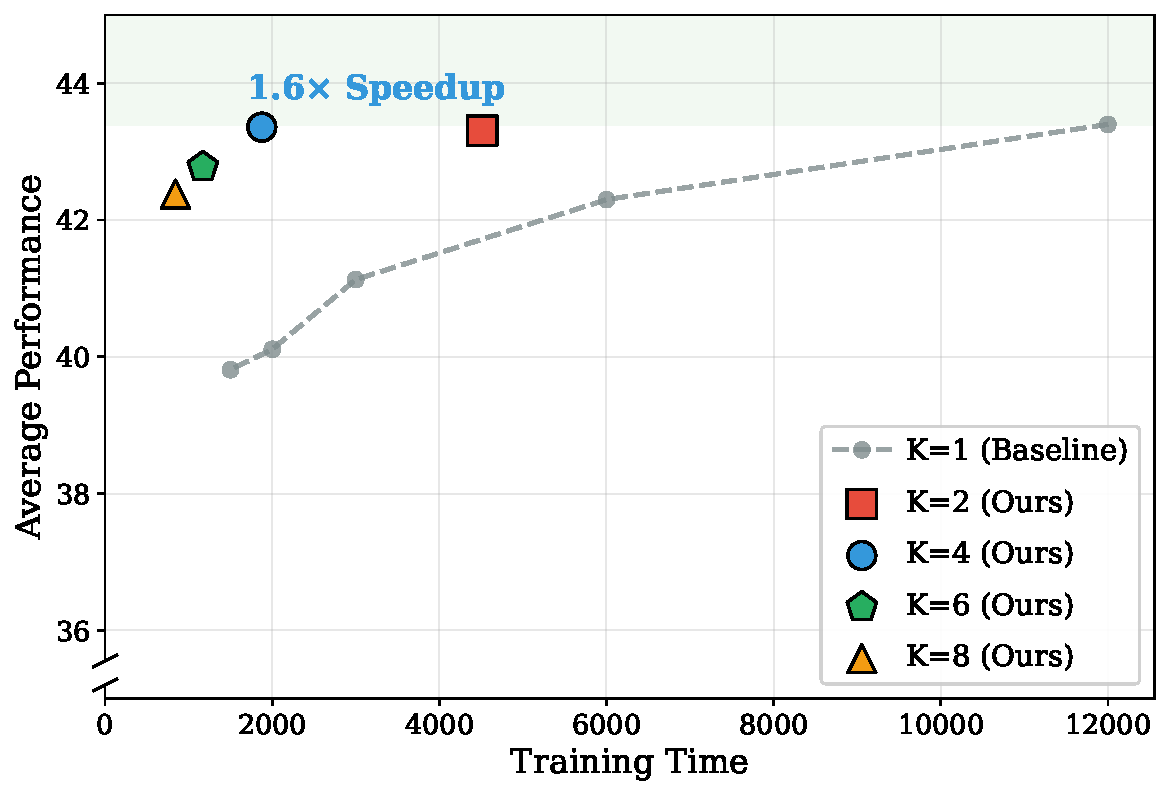
\includegraphics[width=0.9\linewidth]{figures/pareto_main.pdf}
\caption{Training efficiency: Time vs. Performance. The gray dashed line shows $K$=1 baseline performance at different training steps. Our method (colored markers) achieves better performance with significantly less training time.}
\label{fig:pareto_main}
\end{figure}

\paragraph{Ablations}

\begin{table*}[t]
\centering
\caption{Ablation study of complementary masking of \name{} in AR to Diffusion setting.}
\label{tab:ar2diff_complementary_ablation}
\scalebox{0.84}{
\begin{tabular}{lc|ccccccc|c}
\toprule
Method & Complementary & GSM8K & MATH & MMLU & GPQA & IFEval & MBPP & HumanEval & Avg.\\
\midrule
$K$=2 & \cmark & 63.43$_{\pm 1.75}$ & 30.96$_{\pm 0.19}$ & 50.73$_{\pm 0.77}$ & 26.49$_{\pm 0.46}$ & 41.03$_{\pm 1.39}$ & 50.06$_{\pm 1.25}$ & 40.45$_{\pm 3.46}$ & 43.31$_{\pm 0.25}$ \\
$K$=2 & \xmark & 63.36$_{\pm 1.56}$ & 30.10$_{\pm 0.30}$ & 50.91$_{\pm 0.15}$ & 26.41$_{\pm 0.78}$ & 42.82$_{\pm 1.08}$ & 49.42$_{\pm 1.78}$ & 43.29$_{\pm 2.20}$ & 43.76$_{\pm 0.10}$ \\
\midrule
$K$=4 & \cmark & 62.25$_{\pm 0.89}$ & 29.32$_{\pm 0.47}$ & 51.60$_{\pm 0.25}$ & 26.86$_{\pm 0.52}$ & 42.70$_{\pm 1.30}$ & 48.12$_{\pm 0.60}$ & 42.68$_{\pm 1.61}$ & 43.36$_{\pm 0.13}$ \\
$K$=4 & \xmark & 61.58$_{\pm 1.67}$ & 29.11$_{\pm 0.52}$ & 52.21$_{\pm 0.23}$ & 26.12$_{\pm 1.02}$ & 43.90$_{\pm 1.63}$ & 50.59$_{\pm 1.59}$ & 41.16$_{\pm 2.71}$ & 43.52$_{\pm 0.67}$ \\
\bottomrule
\end{tabular}
}
\end{table*}

\paragraph{Gradient Analysis}
We analyze the gradient norm per step for different $K$ settings to understand the optimization dynamics of our method.
As shown in Figure~\ref{fig:gradient_analysis}, we observe that larger $K$ values lead to lower gradient norms per step.
This is because when multiple mask patterns share the same clean context, the gradients from different masked views are aggregated and averaged, resulting in a more stable and smoothed gradient direction.
The reduced gradient variance per step allows for more consistent optimization, which partially explains why our method maintains competitive performance even with fewer training steps.

\begin{figure}[t]
\centering
% TODO: gradient analysis figure
\fbox{\parbox{0.8\linewidth}{\centering\vspace{2em}TODO: Gradient Norm Analysis Figure\vspace{2em}}}
\caption{Gradient norm per step with different $K$ values. Larger $K$ leads to lower gradient norm due to gradient averaging across multiple mask patterns.}
\label{fig:gradient_analysis}
\end{figure}

\subsection{Training Diffusion from Scratch}

For \textbf{Training Diffusion from Scratch}, we follow the experimental settings and framework established by SMDM~\citep{smdm}, using it as our baseline to demonstrate the effectiveness of our approach.

\paragraph{Models}

We train masked diffusion language models from scratch at three different scales: 170M, 336M, and 1028M parameters.
All models are trained on the SlimPajama~\citep{slimpajama} and StarCoder~\citep{starcoder} datasets.
We use a batch size of 256 and a context length of 2048 tokens.
The learning rate is set to $2e-4$ and the learning rate warmup is set to $1\%$ of the total training steps.

\paragraph{Benchmarks}

Following SMDM~\citep{smdm}, we use eight benchmarks covering commonsense reasoning and reading comprehension tasks, including
ARC-e~\citep{arc}, BoolQ~\citep{boolq}, Hellaswag~\citep{hellaswag}, Obqa~\citep{obqa}, PIQA~\citep{piqa}, RACE~\citep{race}, SIQA~\citep{siqa}, LAMBADA~\citep{lambada}.
All benchmarks are evaluated in the zero-shot setting.

\subsection{Speedup Analysis}

We analyze the computational speedup of our context-sharing attention mechanism at both the attention kernel level and the end-to-end training level.
To ensure a fair comparison, we fix the batch size to $4$ and the sequence length to $N = 2048$.
The baseline approach processes $K$ mask patterns independently, resulting in a batch size of $4K$ with sequence length $2N$.
In contrast, our method maintains the same batch size of $4$ but increases the sequence length to $(1+K)N$ by concatenating the shared clean text with $K$ masked texts.

\paragraph{Attention Kernel Speedup}
Our context-sharing attention mask is highly sparse: each masked segment only attends to the shared clean prefix and itself, while remaining isolated from other segments.
By leveraging FlexAttention~\citep{flexattention}, we exploit this sparsity pattern to achieve significant speedup in the attention computation.
As shown in Figure~\ref{fig:attention_speedup}, our sparse attention kernel achieves up to $TODO\times$ speedup compared to dense attention when the number of mask patterns $K$ increases.

\begin{figure}[t]
\centering
% TODO: attention speedup figure
\fbox{\parbox{0.8\linewidth}{\centering\vspace{2em}TODO: Attention Speedup Figure\vspace{2em}}}
\caption{Attention kernel speedup with different number of mask patterns $K$.}
\label{fig:attention_speedup}
\end{figure}

\paragraph{End-to-End Training Speedup}
We measure the end-to-end training speedup by comparing the wall-clock time per training step of our method against the baseline.
As shown in Figure~\ref{fig:e2e_speedup}, our method achieves $TODO\times$ end-to-end training speedup with $K=4$ mask patterns, demonstrating the practical efficiency gains of our approach.

\begin{figure}[t]
\centering
% TODO: end-to-end speedup figure
\fbox{\parbox{0.8\linewidth}{\centering\vspace{2em}TODO: End-to-End Speedup Figure\vspace{2em}}}
\caption{End-to-end training speedup with different number of mask patterns $K$.}
\label{fig:e2e_speedup}
\end{figure}

\input{sections/conclusion}

\section*{Limitations}

% TODO

% \section*{Acknowledgments}
% Acknowledgments should not appear in the review version.

% Bibliography entries for the entire Anthology, followed by custom entries
%\bibliography{anthology,custom}
% Custom bibliography entries only
\bibliography{custom}

\appendix

\section{Theoretical Analysis}

\subsection{Unbiasedness of MMT Loss Estimator}
\label{app:unbiased}

We prove that the MMT training objective is an unbiased estimator of the BDLM objective. Recall that the BDLM loss for a single sample $\mathbf{x}$ is:
\begin{equation}
    \mathcal{L}_{\text{BDLM}}(\mathbf{x}) = -\mathbb{E}_{t, \mathbf{x}^t} \left[ \frac{1}{t} \sum_{i=1}^N \mathbbm{1}[x_i^t = \mathtt{M}] \log p_{\theta}(x_i \mid \mathbf{b}_{<block(i)}, \mathbf{b}_{block(i)}^t) \right],
\end{equation}
where the expectation is over the noise level $t \sim \mathcal{U}(0,1)$ and the stochastic masking process.

\begin{theorem}[Unbiasedness]
\label{thm:unbiased}
Let $\{t_k\}_{k=1}^K$ be $K$ i.i.d. samples from $\mathcal{U}(0,1)$, and let $\{\mathbf{x}^{t_k}\}_{k=1}^K$ be the corresponding independently corrupted sequences. Then:
\begin{equation}
    - \mathbb{E}_{\{t_k\}, \{\mathbf{x}^{t_k}\}} \left[ \frac{1}{K} \sum_{k=1}^K \frac{1}{t_k} \sum_{i=1}^N \mathbbm{1}[x_i^{t_k} = \mathtt{M}] \log p_{\theta}(x_i \mid \mathbf{b}_{<block(i)}, \mathbf{b}_{block(i)}^{t_k}) \right] = \mathcal{L}_{\text{BDLM}}(\mathbf{x}).
\end{equation}
\end{theorem}

\begin{proof}
Define the per-perturbation loss:
\begin{equation}
    \ell_k(\mathbf{x}) \triangleq -\frac{1}{t_k} \sum_{i=1}^N \mathbbm{1}[x_i^{t_k} = \mathtt{M}] \log p_{\theta}(x_i \mid \mathbf{b}_{<block(i)}, \mathbf{b}_{block(i)}^{t_k}).
\end{equation}
By linearity of expectation:
\begin{equation}
    \mathbb{E}\left[ \frac{1}{K} \sum_{k=1}^K \ell_k(\mathbf{x}) \right] = \frac{1}{K} \sum_{k=1}^K \mathbb{E}[\ell_k(\mathbf{x})].
\end{equation}
Since each $(t_k, \mathbf{x}^{t_k})$ is sampled from the same distribution as $(t, \mathbf{x}^t)$ in BDLM:
\begin{equation}
    \mathbb{E}[\ell_k(\mathbf{x})] = \mathbb{E}_{t, \mathbf{x}^t}[\ell(\mathbf{x})] = \mathcal{L}_{\text{BDLM}}(\mathbf{x}), \quad \forall k \in \{1, \ldots, K\}.
\end{equation}
Therefore:
\begin{equation}
    \mathbb{E}\left[ \frac{1}{K} \sum_{k=1}^K \ell_k(\mathbf{x}) \right] = \frac{1}{K} \cdot K \cdot \mathcal{L}_{\text{BDLM}}(\mathbf{x}) = \mathcal{L}_{\text{BDLM}}(\mathbf{x}).
\end{equation}
\end{proof}

\begin{remark}
The key observation is that MMT does not introduce any bias—it simply uses $K$ Monte Carlo samples to estimate the same expected loss as BDLM. The samples share the same clean context $\mathbf{x}$, but each mask pattern is sampled independently, preserving the unbiasedness property.
\end{remark}

However, this comparison is misleading because BDLM requires $K$ forward passes while MMT only requires 1 forward pass (with efficient context sharing). When computational cost is properly accounted for, MMT achieves better variance-to-compute ratio by reducing mask noise through averaging, while maintaining training efficiency via context reuse.


\end{document}
